\documentclass[working]{article}

% Chinese support (load before preamble)
\usepackage{ctex}

% Configure natbib for report (use author-year style)
% This must be done before loading preamble
\PassOptionsToPackage{authoryear,round}{natbib}

% Style settings for beamer slides
% Referenced from research-collection/preamble.tex
% Note: ctex and tikz should be loaded before this preamble (in slides.tex)

% Configure natbib for Beamer (use numbers instead of author-year)
% This must be done before loading preamble_base.tex
\PassOptionsToPackage{numbers,sort&compress}{natbib}
\PassOptionsToPackage{most,many,breakable}{tcolorbox}

% Basic packages and settings for all outputs
% This file contains common packages used across manuscript, report, and slides

% Essential packages
\usepackage{amsmath}        % Advanced math formatting
\usepackage{amssymb}        % Advanced math symbols
\usepackage{amsthm}         % Theorem environments
\usepackage{graphicx}       % Graphics support
\usepackage{hyperref}       % Hyperlinks
\usepackage{booktabs}       % Professional tables
\usepackage{float}          % Better float control
\usepackage{xcolor}         % Color support
\usepackage{microtype}      % Better typography
\usepackage{bm}             % Bold math
\usepackage{subcaption}     % Subfigure environment
\usepackage{natbib}         % Advanced citation management
\usepackage{caption}        % Caption formatting
\usepackage{tcolorbox}
\usepackage{xparse}         % Enhanced command definitions
\usepackage[ruled,vlined,linesnumbered]{algorithm2e} % Algorithm environment

% Hyperref settings
% Note: research-collection does not use colorlinks, so links appear as boxes instead of colored text
% Uncomment the following to use colored links:
% \hypersetup{
%     colorlinks,
%     linkcolor=blue,
%     citecolor=black,
%     urlcolor=blue!80!black
% }

% Caption settings
\captionsetup[figure]{labelfont=bf, labelsep=period, name={Figure}}
\captionsetup[table]{labelfont=bf, labelsep=period, name={Table}}

% Cross-reference settings
\usepackage{cleveref}       % Smart cross-references
\Crefname{figure}{Figure}{Figures}
\crefname{figure}{Figure}{Figures}
\Crefname{table}{Table}{Tables}
\crefname{table}{Table}{Tables}
\Crefname{equation}{Equation}{Equations}
\crefname{equation}{Equation}{Equations}

%%%%%%%%%%%%%%%%%%%%%%%%%%%%%%%%%%%%%%%%%%%%%%%%%%%%%%%%%%%%%%%%%%%%%%%%%%%%%%%
%  Simple and Useful Symbol Definitions                                        %
%%%%%%%%%%%%%%%%%%%%%%%%%%%%%%%%%%%%%%%%%%%%%%%%%%%%%%%%%%%%%%%%%%%%%%%%%%%%%%%

% Symbol aliases (common mathematical notation shortcuts)
\let\implies\Rightarrow
\let\impliedby\Leftarrow
\let\iff\Leftrightarrow
\let\epsilon\varepsilon

% Math operators
\DeclareMathOperator*{\argmax}{\arg\!max}
\DeclareMathOperator*{\argmin}{\arg\!min}
\DeclareMathOperator*{\vperp}{\text{\rotatebox{90}{$\models$}}}

% Paired delimiters and norms (requires mathtools)
\RequirePackage{mathtools}
\DeclarePairedDelimiterX{\infdivx}[2]{(}{)}{%
  #1\;\delimsize\|\;#2%
}
\DeclarePairedDelimiter{\norm}{\lVert}{\rVert}

% Common math commands
\newcommand{\E}{\mathbb{E}}
\newcommand{\infdiv}{D_{\mathbb{KL}}\infdivx}
\newcommand{\fisherdiv}{D_{\mathbb{F}}\infdivx}

% Simple utility commands
\newcommand*\widefbox[1]{\fbox{\hspace{2em}#1\hspace{2em}}}



% Custom counter for figure placeholder items
\newcounter{figureplaceholderitem}
\renewcommand{\thefigureplaceholderitem}{\Alph{figureplaceholderitem}}

% Custom item command that takes optional name
\newcommand{\figureplaceholderitem}[1][]{%
    \stepcounter{figureplaceholderitem}%
    \par\noindent\textbf{\thefigureplaceholderitem.}%
    \ifx\relax#1\relax%
    \else%
        \textbf{ #1}%
    \fi%
    \space
}

% Helper command for item in figureplaceholder environment
% Use xparse for more robust optional argument handling
\makeatletter
% Use xparse for better compatibility with enumitem
\NewDocumentCommand{\@figureplaceholderitemcmd}{o}{%
    \IfValueTF{#1}{%
        \figureplaceholderitem[#1]%
    }{%
        \figureplaceholderitem[]%
    }%
}
\makeatother

% Custom environment for figure placeholders
\makeatletter
\newtcolorbox{figureplaceholder}{
    fontupper=\footnotesize,
    boxrule=0.5pt,
    colback=white,
    colframe=black,
    left=5pt,
    right=5pt,
    top=5pt,
    bottom=5pt,
    before upper={%
        \linespread{1}\selectfont%
        \setcounter{figureplaceholderitem}{0}%
        \let\olditem\item%
        \let\item\@figureplaceholderitemcmd%
    },
    after upper={%
        \let\item\olditem%
        \setcounter{figureplaceholderitem}{0}%
    }
}
\makeatother

% Additional packages for slides
\usepackage[T1]{fontenc}
\usepackage[utf8]{inputenc}
\usepackage{framed}
\usepackage{multicol}
\usepackage{ragged2e}
\justifying\let\raggedright\justifying
\usepackage[export]{adjustbox}
\usepackage{latexsym}
\usepackage{calligra}
\usepackage{pstricks}
\usepackage{listings}
\usepackage{stackengine}
\usepackage{makecell}
\usepackage{CUHK}  % CUHK beamer theme with purple header, golden title, and navigation dots
\usepackage{pifont}
\usepackage{ulem}
\usepackage{empheq}
\usepackage[font=scriptsize]{caption}
\usepackage{advdate}
\usepackage{extarrows}
\usepackage{bbm}

% Additional symbol definitions (base preamble has common ones)
% Slides-specific symbols
\newcommand{\cmark}{\ding{51}}%
\newcommand{\xmark}{\ding{55}}%
\DeclareMathOperator*{\mean}{mean}
\DeclareMathOperator*{\diag}{diag}

% User-defined commands
\def\cmd#1{\texttt{\color{red}\footnotesize $\backslash$#1}}
\def\env#1{\texttt{\color{blue}\footnotesize #1}}
\def\ulbf#1{\textbf{\underline{#1}}}
\def\todo#1{\large\color{red}\textit{#1}}

% Listings settings (matching research-collection style)
\xdefinecolor{cuhk1}{rgb}{0.457,0.0585,0.42578}      %RGB(117,15,109)
\xdefinecolor{cuhk2}{rgb}{0.86328,0.63671875,0}      %RGB(221,163,0)
\xdefinecolor{cuhk3}{rgb}{0.953125,0.87109,0.6875}   %RGB(244,223,176)

\definecolor{deepred}{rgb}{0.6,0,0}
\definecolor{frenchblue}{rgb}{0.0, 0.25, 0.63}

%%%%%%%%%%%%%%%%%%%%%%%%%%%%%%%%%%%%%%%%%%%%%%%%%%%%%%%%%%%%%%%%%%%%%%%%%%%%%%%
%                           Beamer Theorem Environments                       %
%%%%%%%%%%%%%%%%%%%%%%%%%%%%%%%%%%%%%%%%%%%%%%%%%%%%%%%%%%%%%%%%%%%%%%%%%%%%%%%

% Additional packages for theorem environments in Beamer
\usepackage{thmtools}
\tcbuselibrary{theorems,skins,hooks}
\usetikzlibrary{arrows,calc,shadows.blur}

% Base colors harmonized with CUHK theme
\definecolor{cuhkpurple}{RGB}{117, 15, 109}    % CUHK primary purple
\definecolor{cuhkgold}{RGB}{221, 163, 0}       % CUHK gold
\definecolor{cuhkbeige}{RGB}{244, 223, 176}    % CUHK beige

% Theme colors (harmonized palette)
\definecolor{myblue}{RGB}{45, 111, 177}        % Complementary blue
\definecolor{mygreen}{RGB}{56, 140, 70}        % Nature green
\definecolor{myorange}{RGB}{255, 140, 0}      % Warm orange
\definecolor{mypurple}{RGB}{117, 15, 109}      % Matching CUHK purple
\definecolor{myteal}{RGB}{0, 128, 128}         % Teal accent

% Environment colors (harmonized with theme - softened for subtlety)
\colorlet{theorem}{cuhkpurple!65!black}       % Soft purple for theorems
\colorlet{lemma}{cuhkpurple!55!blue}          % Soft purple-blue for lemmas
\colorlet{corollary}{cuhkpurple!50!mypurple}  % Soft purple variant for corollaries
\colorlet{prop}{cuhkpurple!60!black}          % Soft purple for propositions
\colorlet{claim}{myteal!60!black}             % Soft teal for claims
\colorlet{definition}{mygreen!60!black}       % Soft green for definitions
\colorlet{example}{cuhkgold!65!black}        % Soft gold for examples
\colorlet{exercise}{myorange!55!black}       % Soft orange for exercises
\colorlet{proof}{theorem}                     % Same as theorem

% Override Beamer's default theorem environment styling with tcolorbox
% Using tcolorbox blocks that work well with Beamer
\makeatletter

% Custom theorem-like environments using tcolorbox blocks
\newtcolorbox{tcbtheorem}[1][]{
    enhanced,
    breakable,
    parbox=false,
    before skip=2mm plus 0.5mm minus 0.5mm,
    after skip=2mm plus 0.5mm minus 0.5mm,
    colback=theorem!4,
    colframe=theorem!70!black,
    colbacktitle=theorem!65!black,
    coltitle=white,
    boxrule=1.2pt,
    arc=4pt,
    left=4mm,
    right=4mm,
    top=3mm,
    bottom=3mm,
    fonttitle=\bfseries\sffamily,
    attach boxed title to top left={
        xshift=4mm,
        yshift*=-2mm
    },
    boxed title style={
        enhanced,
        colback=theorem!65!black,
        arc=4pt,
        boxrule=0pt
    },
    title=\textbf{Theorem\ifx\relax#1\relax\else: #1\fi}
}

\newtcolorbox{tcblemma}[1][]{
    enhanced,
    breakable,
    parbox=false,
    before skip=2mm plus 0.5mm minus 0.5mm,
    after skip=2mm plus 0.5mm minus 0.5mm,
    colback=lemma!4,
    colframe=lemma!70!black,
    colbacktitle=lemma!65!black,
    coltitle=white,
    boxrule=1.2pt,
    arc=4pt,
    left=4mm,
    right=4mm,
    top=3mm,
    bottom=3mm,
    fonttitle=\bfseries\sffamily,
    attach boxed title to top left={
        xshift=4mm,
        yshift*=-2mm
    },
    boxed title style={
        enhanced,
        colback=lemma!65!black,
        arc=4pt,
        boxrule=0pt
    },
    title=\textbf{Lemma\ifx\relax#1\relax\else: #1\fi}
}

\newtcolorbox{tcbcorollary}[1][]{
    enhanced,
    breakable,
    parbox=false,
    before skip=2mm plus 0.5mm minus 0.5mm,
    after skip=2mm plus 0.5mm minus 0.5mm,
    colback=corollary!4,
    colframe=corollary!70!black,
    colbacktitle=corollary!65!black,
    coltitle=white,
    boxrule=1.2pt,
    arc=4pt,
    left=4mm,
    right=4mm,
    top=3mm,
    bottom=3mm,
    fonttitle=\bfseries\sffamily,
    attach boxed title to top left={
        xshift=4mm,
        yshift*=-2mm
    },
    boxed title style={
        enhanced,
        colback=corollary!65!black,
        arc=4pt,
        boxrule=0pt
    },
    title=\textbf{Corollary\ifx\relax#1\relax\else: #1\fi}
}

\newtcolorbox{tcbprop}[1][]{
    enhanced,
    breakable,
    parbox=false,
    before skip=2mm plus 0.5mm minus 0.5mm,
    after skip=2mm plus 0.5mm minus 0.5mm,
    colback=prop!4,
    colframe=prop!70!black,
    colbacktitle=prop!65!black,
    coltitle=white,
    boxrule=1.2pt,
    arc=4pt,
    left=4mm,
    right=4mm,
    top=3mm,
    bottom=3mm,
    fonttitle=\bfseries\sffamily,
    attach boxed title to top left={
        xshift=4mm,
        yshift*=-2mm
    },
    boxed title style={
        enhanced,
        colback=prop!65!black,
        arc=4pt,
        boxrule=0pt
    },
    title=\textbf{Proposition\ifx\relax#1\relax\else: #1\fi}
}

\newtcolorbox{tcbclaim}[1][]{
    enhanced,
    breakable,
    parbox=false,
    before skip=2mm plus 0.5mm minus 0.5mm,
    after skip=2mm plus 0.5mm minus 0.5mm,
    colback=claim!4,
    colframe=claim!70!black,
    colbacktitle=claim!65!black,
    coltitle=white,
    boxrule=1.2pt,
    arc=4pt,
    left=4mm,
    right=4mm,
    top=3mm,
    bottom=3mm,
    fonttitle=\bfseries\sffamily,
    attach boxed title to top left={
        xshift=4mm,
        yshift*=-2mm
    },
    boxed title style={
        enhanced,
        colback=claim!65!black,
        arc=4pt,
        boxrule=0pt
    },
    title=\textbf{Claim\ifx\relax#1\relax\else: #1\fi}
}

\newtcolorbox{tcbdefinition}[1][]{
    enhanced,
    breakable,
    parbox=false,
    before skip=2mm plus 0.5mm minus 0.5mm,
    after skip=2mm plus 0.5mm minus 0.5mm,
    colback=definition!3,
    colframe=definition!70!black,
    colbacktitle=definition!65!black,
    coltitle=white,
    boxrule=1.2pt,
    arc=4pt,
    left=4mm,
    right=4mm,
    top=3mm,
    bottom=3mm,
    fonttitle=\bfseries\sffamily,
    attach boxed title to top left={
        xshift=4mm,
        yshift*=-2mm
    },
    boxed title style={
        enhanced,
        colback=definition!65!black,
        arc=4pt,
        boxrule=0pt
    },
    title=\textbf{Definition\ifx\relax#1\relax\else: #1\fi}
}

\newtcolorbox{tcbexample}[1][]{
    enhanced,
    breakable,
    parbox=false,
    before skip=2mm plus 0.5mm minus 0.5mm,
    after skip=2mm plus 0.5mm minus 0.5mm,
    colback=example!5,
    colframe=example!70!black,
    colbacktitle=example!65!black,
    coltitle=white,
    boxrule=1.5pt,
    arc=4pt,
    left=4mm,
    right=4mm,
    top=3mm,
    bottom=3mm,
    fonttitle=\bfseries\sffamily,
    attach boxed title to top left={
        xshift=4mm,
        yshift*=-2mm
    },
    boxed title style={
        enhanced,
        colback=example!65!black,
        arc=4pt,
        boxrule=0pt
    },
    title=\textbf{Example\ifx\relax#1\relax\else: #1\fi}
}

\newtcolorbox{tcbexercise}[1][]{
    enhanced,
    breakable,
    parbox=false,
    before skip=2mm plus 0.5mm minus 0.5mm,
    after skip=2mm plus 0.5mm minus 0.5mm,
    colback=exercise!4,
    colframe=exercise!70!black,
    colbacktitle=exercise!65!black,
    coltitle=white,
    boxrule=1.2pt,
    arc=4pt,
    left=4mm,
    right=4mm,
    top=3mm,
    bottom=3mm,
    fonttitle=\bfseries\sffamily,
    attach boxed title to top left={
        xshift=4mm,
        yshift*=-2mm
    },
    boxed title style={
        enhanced,
        colback=exercise!65!black,
        arc=4pt,
        boxrule=0pt
    },
    title=\textbf{Exercise\ifx\relax#1\relax\else: #1\fi}
}

\newtcolorbox{tcbquestion}[1][]{
    enhanced,
    breakable,
    before skip=2mm,
    after skip=2mm,
    colback=myblue!3,
    colframe=myblue!70!black,
    colbacktitle=myblue!65!black,
    coltitle=white,
    boxrule=1.2pt,
    arc=4pt,
    left=4mm,
    right=4mm,
    top=3mm,
    bottom=3mm,
    fonttitle=\bfseries\sffamily,
    attach boxed title to top left={
        xshift=4mm,
        yshift*=-2mm
    },
    boxed title style={
        enhanced,
        colback=myblue!65!black,
        arc=4pt,
        boxrule=0pt
    },
    title=\textbf{Question\ifx\relax#1\relax\else: #1\fi}
}

\newtcolorbox{tcbsolution}[1][]{
    enhanced,
    breakable,
    before skip=2mm,
    after skip=2mm,
    colback=definition!4,
    colframe=definition!70!black,
    boxrule=0pt,
    leftrule=2pt,
    rightrule=0pt,
    toprule=0pt,
    bottomrule=0pt,
    arc=3pt,
    left=8mm,
    right=4mm,
    top=2mm,
    bottom=2mm,
    fonttitle=\bfseries\sffamily\color{definition!70!black},
    title={\textbf{Solution\ifx\relax#1\relax\else: #1\fi}}
}

% Note - Beamer has a default note environment, so we create a custom one
\newtcolorbox{notebox}[1][]{%
    enhanced,
    colback=cuhkbeige!10,%
    colframe=cuhkbeige!55!black,
    size=small,
    boxrule=1.2pt,
    arc=4pt,
    title=\textbf{Note},
    halign title=flush left,
    coltitle=cuhkpurple!65!black,
    breakable,
    parbox=false,
    before skip=2mm plus 0.5mm minus 0.5mm,
    after skip=2mm plus 0.5mm minus 0.5mm,
    left=3mm,
    right=3mm,
    top=2mm,
    bottom=2mm,
    #1,
}

% Proof - Beamer has a default proof environment, so we create a custom one with vertical line style
\newtcolorbox{proofbox}[1][]{
    enhanced,
    breakable,
    parbox=false,
    before skip=2mm plus 0.5mm minus 0.5mm,
    after skip=2mm plus 0.5mm minus 0.5mm,
    colback=proof!4,
    colframe=proof!70!black,
    boxrule=0pt,
    leftrule=2pt,
    rightrule=0pt,
    toprule=0pt,
    bottomrule=0pt,
    arc=3pt,
    left=8mm,
    right=4mm,
    top=2mm,
    bottom=2mm,
    before upper={\textbf{\textcolor{proof!70!black}{Proof\ifx\relax#1\relax\else: #1\fi}}\par\vspace{-2mm}},
    #1
}

\newtcolorbox{explanation}[1][]{
    enhanced,
    breakable,
    parbox=false,
    before skip=2mm plus 0.5mm minus 0.5mm,
    after skip=2mm plus 0.5mm minus 0.5mm,
    colback=example!4,
    colframe=example!70!black,
    boxrule=0pt,
    leftrule=2pt,
    rightrule=0pt,
    toprule=0pt,
    bottomrule=0pt,
    arc=3pt,
    left=8mm,
    right=4mm,
    top=2mm,
    bottom=2mm,
    fonttitle=\bfseries\sffamily\color{example!70!black},
    title={\textbf{Explanation\ifx\relax#1\relax\else: #1\fi}}
}

% Note: Beamer already defines 'note' environment, so we don't redefine it
% Use \begin{notebox}...\end{notebox} directly if you need the custom styled note box
% Beamer's note environment is used for speaker notes, so we don't override it

% Redefine proof environment using proofbox with title option support
\RenewDocumentEnvironment{proof}{O{}}{%
    \begin{proofbox}[#1]
}{%
    \end{proofbox}
}

% Redefine standard beamer theorem environments to use tcolorbox
% Beamer's theorem environments are block-based, so we'll use tcolorbox blocks
% Pass the optional argument directly to tcolorbox, which will use it as the title suffix
\RenewDocumentEnvironment{theorem}{O{}}{%
    \begin{tcbtheorem}[#1]
}{%
    \end{tcbtheorem}
}

\RenewDocumentEnvironment{lemma}{O{}}{%
    \begin{tcblemma}[#1]
}{%
    \end{tcblemma}
}

\RenewDocumentEnvironment{corollary}{O{}}{%
    \begin{tcbcorollary}[#1]
}{%
    \end{tcbcorollary}
}

% prop, claim, exercise are not standard Beamer environments, so we use NewDocumentEnvironment
\NewDocumentEnvironment{prop}{O{}}{%
    \begin{tcbprop}[#1]
}{%
    \end{tcbprop}
}

\NewDocumentEnvironment{claim}{O{}}{%
    \begin{tcbclaim}[#1]
}{%
    \end{tcbclaim}
}

\RenewDocumentEnvironment{definition}{O{}}{%
    \begin{tcbdefinition}[#1]
}{%
    \end{tcbdefinition}
}

\RenewDocumentEnvironment{example}{O{}}{%
    \begin{tcbexample}[#1]
}{%
    \end{tcbexample}
}

\NewDocumentEnvironment{exercise}{O{}}{%
    \begin{tcbexercise}[#1]
}{%
    \end{tcbexercise}
}

\NewDocumentEnvironment{question}{O{}}{%
    \begin{tcbquestion}[#1]
}{%
    \end{tcbquestion}
}

% Solution environment - check if already defined
\@ifundefined{solution}{%
    \NewDocumentEnvironment{solution}{O{}}{%
        \begin{tcbsolution}[#1]
    }{%
        \end{tcbsolution}
    }
}{%
    \RenewDocumentEnvironment{solution}{O{}}{%
        \begin{tcbsolution}[#1]
    }{%
        \end{tcbsolution}
    }
}

\makeatother

\lstset{
    basicstyle=\ttfamily\small,
    keywordstyle=\bfseries\color{cuhk1},
    emphstyle=\ttfamily\color{deepred},
    stringstyle=\color{cuhk2},
    numbers=left,
    numberstyle=\small\color{cuhk3},
    rulesepcolor=\color{red!20!green!20!blue!20},
    frame=shadowbox,
}

%%%%%%%%%%%%%%%%%%%%%%%%%%%%%%%%%%%%%%%%%%%%%%%%%%%%%%%%%%%%%%%%%%%%%%%%%%%%%%%
%  Generic Reusable Blocks Based on Colors and Styles                         %
%%%%%%%%%%%%%%%%%%%%%%%%%%%%%%%%%%%%%%%%%%%%%%%%%%%%%%%%%%%%%%%%%%%%%%%%%%%%%%%

% Generic tcolorbox with vertical line style (left border only)
% Usage: \begin{vertlineblock}[color]{title}...\end{vertlineblock}
% Example: \begin{vertlineblock}[myorange]{Important Note}...\end{vertlineblock}
\newtcolorbox{vertlineblock}[2][]{
  enhanced,
  breakable,
  parbox=false,
  before skip=2mm plus 0.5mm minus 0.5mm,
  after skip=2mm plus 0.5mm minus 0.5mm,
  colback=#1!4,
  colframe=#1!70!black,
  boxrule=0pt,
  leftrule=2pt,
  rightrule=0pt,
  toprule=0pt,
  bottomrule=0pt,
  arc=3pt,
  left=8mm,
  right=4mm,
  top=2mm,
  bottom=2mm,
  fonttitle=\bfseries\sffamily\color{#1!70!black},
  title={#2}
}

% Generic tcolorbox with full border style
% Usage: \begin{fullborderblock}[color]{title}...\end{fullborderblock}
% Example: \begin{fullborderblock}[cuhkgold]{Key Point}...\end{fullborderblock}
\newtcolorbox{fullborderblock}[2][]{
  enhanced,
  breakable,
  parbox=false,
  before skip=2mm plus 0.5mm minus 0.5mm,
  after skip=2mm plus 0.5mm minus 0.5mm,
  colback=#1!5,
  colframe=#1!70!black,
  boxrule=2pt,
  arc=3pt,
  left=4mm,
  right=4mm,
  top=2mm,
  bottom=2mm,
  fonttitle=\bfseries\sffamily\color{#1!70!black},
  title={#2}
}

% Generic tcolorbox with title box style (colored title box attached to top)
% Usage: \begin{titleboxblock}[color]{title}...\end{titleboxblock}
% Example: \begin{titleboxblock}[mygreen]{Key Concept}...\end{titleboxblock}
\newtcolorbox{titleboxblock}[2][]{
  enhanced,
  breakable,
  parbox=false,
  before skip=2mm plus 0.5mm minus 0.5mm,
  after skip=2mm plus 0.5mm minus 0.5mm,
  colback=#1!3,
  colframe=#1!70!black,
  colbacktitle=#1!65!black,
  coltitle=white,
  boxrule=1.2pt,
  arc=4pt,
  left=4mm,
  right=4mm,
  top=2mm,
  bottom=2mm,
  attach boxed title to top left={
    xshift=4mm,
    yshift*=-2mm
  },
  varwidth boxed title*=-3cm,
  boxed title style={
    enhanced,
    colback=#1!65!black,
    arc=4pt,
    interior style={fill=#1!65!black}
  },
  fonttitle=\bfseries\sffamily,
  title={#2},
  left=4mm,
  right=4mm,
  top=2mm,
  bottom=2mm
}

% Generic highlight block with optional title
% Usage: \begin{highlightblock}[color]{title}...\end{highlightblock}
%        or \begin{highlightblock}[color]{}...\end{highlightblock} (no title)
% Example: \begin{highlightblock}[myblue]{Reminder}...\end{highlightblock}
% Note: Title uses white text on colored background for better contrast
\newtcolorbox{highlightblock}[2][]{
  enhanced,
  breakable,
  parbox=false,
  before skip=2mm plus 0.5mm minus 0.5mm,
  after skip=2mm plus 0.5mm minus 0.5mm,
  colback=#1!4,
  colframe=#1!70!black,
  colbacktitle=#1!65!black,
  coltitle=white,
  boxrule=1.2pt,
  arc=4pt,
  left=4mm,
  right=4mm,
  top=2mm,
  bottom=2mm,
  fonttitle=\bfseries\sffamily,
  attach boxed title to top left={
    xshift=4mm,
    yshift*=-2mm
  },
  boxed title style={
    enhanced,
    colback=#1!65!black,
    arc=4pt,
    boxrule=0pt
  },
  title={#2}
}

% Convenience environments using predefined colors
% Vertical line style blocks (left border only, like Exercise and Proof)
% Usage: \begin{purplevertblock}{title}...\end{purplevertblock}
\NewDocumentEnvironment{purplevertblock}{O{}}{%
  \begin{vertlineblock}[cuhkpurple]{#1}
}{%
  \end{vertlineblock}
}

\NewDocumentEnvironment{goldvertblock}{O{}}{%
  \begin{vertlineblock}[cuhkgold]{#1}
}{%
  \end{vertlineblock}
}

\NewDocumentEnvironment{greenvertblock}{O{}}{%
  \begin{vertlineblock}[mygreen]{#1}
}{%
  \end{vertlineblock}
}

\NewDocumentEnvironment{bluevertblock}{O{}}{%
  \begin{vertlineblock}[myblue]{#1}
}{%
  \end{vertlineblock}
}

\NewDocumentEnvironment{orangevertblock}{O{}}{%
  \begin{vertlineblock}[myorange]{#1}
}{%
  \end{vertlineblock}
}

% Title box style blocks (colored title box, like Definition)
% Usage: \begin{purpletitleblock}{title}...\end{purpletitleblock}
\NewDocumentEnvironment{purpletitleblock}{O{}}{%
  \begin{titleboxblock}[cuhkpurple]{#1}
}{%
  \end{titleboxblock}
}

\NewDocumentEnvironment{goldtitleblock}{O{}}{%
  \begin{titleboxblock}[cuhkgold]{#1}
}{%
  \end{titleboxblock}
}

\NewDocumentEnvironment{greentitleblock}{O{}}{%
  \begin{titleboxblock}[mygreen]{#1}
}{%
  \end{titleboxblock}
}

\NewDocumentEnvironment{bluetitleblock}{O{}}{%
  \begin{titleboxblock}[myblue]{#1}
}{%
  \end{titleboxblock}
}

% Full border style blocks (all sides, like Example)
% Usage: \begin{goldborderblock}{title}...\end{goldborderblock}
\NewDocumentEnvironment{goldborderblock}{O{}}{%
  \begin{fullborderblock}[cuhkgold]{#1}
}{%
  \end{fullborderblock}
}

\NewDocumentEnvironment{purpleborderblock}{O{}}{%
  \begin{fullborderblock}[cuhkpurple]{#1}
}{%
  \end{fullborderblock}
}

% Override figure/table names for English in Chinese documents
\renewcommand{\figurename}{Figure}
\renewcommand{\tablename}{Table}
\renewcommand{\refname}{References}

% Additional command for date advancement
\newcommand{\advanceday}[1][14]{
\begingroup
\AdvanceDate[#1]
\today
\endgroup
}



\geometry{a4paper,left=2cm,right=6cm,top=2cm,bottom=2cm}
\setlength{\marginparwidth}{4cm}
% \linenumbers

% Bibliography style for report (author-year style)
\bibliographystyle{abbrvnat}
\setcitestyle{authoryear, open={(},close={)}}

\title{Weekly Report of Learning Notes}
\author{Your Name}
\date{\today}

\begin{document}

\maketitle
\tableofcontents

\section{Weekly Summary}

测试中文支持

This is an example weekly report generated from the template.
The report can integrate multiple drafts from the \texttt{drafts/} directory.

% Import drafts
% Example: \input{../drafts/20241013-diffusionmodel.tex}
% \input{../drafts/<timestamp>_<short_desc>.tex}

\section{Progress}

\begin{itemize}
    \item Completed template structure setup\citep{example2024}.
    \item Tested compilation scripts\citet{example2024}.
    \item Verified all document types work correctly\cite{example2024}.
\end{itemize}

% Import example draft demonstrating all special environments
% Example draft file demonstrating all special environments
% Date: 2025-11-01
% This file can be included in reports using % Example draft file demonstrating all special environments
% Date: 2025-11-01
% This file can be included in reports using % Example draft file demonstrating all special environments
% Date: 2025-11-01
% This file can be included in reports using \input{../drafts/20251101_example_draft.tex}

\section{Example Draft: Special Environments}

This draft demonstrates the use of various special environments available in the template,
including definitions, theorems, lemmas, and other mathematical environments.

\subsection{Definition}

\begin{definition}[Important Concept]
A definition environment can be used to introduce key concepts.
The template provides colored definition boxes when using the \texttt{working} class option.
\end{definition}

\begin{definition}
This is a definition without a title.
\end{definition}

\subsection{Theorem Environments}

\begin{theorem}[Fundamental Theorem]
This is a theorem statement. The theorem environment is automatically numbered within sections.
\end{theorem}

\begin{lemma}[Key Lemma]
This is a lemma. Lemmas are typically used to prove theorems.
\end{lemma}

\begin{corollary}[Important Result]
This is a corollary that follows from the theorem above.
\end{corollary}

\begin{prop}[Useful Proposition]
This is a proposition statement.
\end{prop}

\begin{claim}[Test Claim]
This is a claim that needs to be verified.
\end{claim}

\subsection{Examples and Exercises}

\begin{example}
This is an example demonstrating how to use the example environment.
Examples are useful for illustrating concepts.
\end{example}

\begin{exercise}
This is an exercise for the reader to complete.
Exercises can be used in teaching materials or practice problems.
\end{exercise}

\subsection{Questions and Solutions}

\begin{question}
What is the purpose of this template?
\end{question}

\begin{solution}
The template provides a structured way to create multiple document types (manuscripts, reports, slides) from a single content base.
\end{solution}

\subsection{Proof Environments}

\begin{proof}
This is a proof environment. The proof will automatically end with a QED symbol (or custom symbol defined in the preamble).
The template uses a smiley face as the QED symbol by default.
\end{proof}

\begin{explanation}
This is an explanation environment, similar to proof but with different styling.
It can be used to provide detailed explanations of concepts.
\end{explanation}

\subsection{Other Environments}

\begin{note}
This is a note environment for additional remarks or observations.
Notes are typically styled with a gray background.
\end{note}

\subsection{Mathematical Notation}

The template includes custom mathematical commands:

\begin{itemize}
    \item KL divergence: $\infdiv{P}{Q}$ where $P$ and $Q$ are probability distributions
    \item Norm: $\norm{\mathbf{x}}$ for vector norms
    \item Expectation: $\E[X]$ for expected value
    \item Operators: $\argmax$, $\argmin$, $\vperp$ for perpendicular
\end{itemize}

\subsection{Code Listings}

The template supports code listings with syntax highlighting:

\begin{lstlisting}[language=Python]
def example_function(x, y):
    """Example Python function"""
    result = x + y
    return result
\end{lstlisting}

\begin{lstlisting}[language=R]
# Example R code
x <- c(1, 2, 3, 4, 5)
mean(x)
\end{lstlisting}

\subsection{Algorithms}

The template supports algorithm environments:

\begin{algorithm}[H]
\caption{Example Algorithm}
\Initialize{Set initial parameters}
\For{each iteration}{
    \State Compute value
    \If{condition is met}{
        \State Return result
    }
}
\end{algorithm}

\subsection{Framed Environments}

The template provides framed environments for emphasis:

\begin{framed}
This text is in a framed box, useful for highlighting important information.
\end{framed}

\subsection{Custom Commands}

The template includes several custom commands:
\begin{itemize}
    \item \cmd{commandname} - formats command names in red
    \item \env{envname} - formats environment names in blue
    \item \ulbf{bold underline} - creates bold underlined text
    \item \todo{reminder} - creates red italic todo notes
\end{itemize}

\subsection{Special Symbols}

The template provides checkmark and cross symbols:
\begin{itemize}
    \item \cmark{} - checkmark symbol
    \item \xmark{} - cross symbol
\end{itemize}

\subsection{Summary}

This example draft demonstrates the comprehensive set of environments and commands available in the template.
All these environments work seamlessly in reports and can be adapted for manuscripts and slides as needed.

\section{Generic Reusable Blocks}

You can use generic blocks with custom titles and colors for highlighting any content. These blocks are named by style (vertical line, title box, full border) and can be used with any color:

\begin{purplevertblock}{Important Note}
This block uses vertical line style (left border only) with purple color.
This is the same style used by \texttt{exercise} and \texttt{proof} environments.
Perfect for important notes or reminders.
\end{purplevertblock}

\begin{orangevertblock}{Exercise-Style Block}
This demonstrates the vertical line style with orange color, matching the exercise environment style.
\begin{enumerate}
    \item First item in the list
    \item Second item
    \item Works great with enumerate and itemize!
\end{enumerate}
\end{orangevertblock}

\begin{goldtitleblock}{Key Concept}
This block uses the title box style (colored title box at top) with gold color.
This is the same style used by \texttt{definition} environment.
Perfect for definitions or key concepts.
\end{goldtitleblock}

\begin{goldborderblock}{Important Warning}
This block has a full border (all sides) with gold color.
This is the same style used by \texttt{example} environment.
Useful for warnings or critical information.
\end{goldborderblock}

\begin{highlightblock}[myblue]{Custom Highlight}
You can use \texttt{highlightblock} with any color for flexible highlighting:
\begin{verbatim}
\begin{highlightblock}[myblue]{Title}
Content here...
\end{highlightblock}
\end{verbatim}
This works great for code examples, lists, or any content you want to emphasize.
\end{highlightblock}

\begin{vertlineblock}[mygreen]{Generic Vertical Line Block}
Use \texttt{vertlineblock} with any color name for a vertical line style:
\begin{verbatim}
\begin{vertlineblock}[mygreen]{Title}
Content with lists:
\begin{itemize}
    \item Item 1
    \item Item 2
\end{itemize}
\end{vertlineblock}
\end{verbatim}
\end{vertlineblock}

\begin{titleboxblock}[cuhkpurple]{Generic Title Box Block}
Use \texttt{titleboxblock} with any color name for a title box style:
\begin{verbatim}
\begin{titleboxblock}[cuhkpurple]{Title}
Any content including equations:
\begin{equation}
E = mc^2
\end{equation}
\end{titleboxblock}
\end{verbatim}
\end{titleboxblock}

These generic blocks are fully flexible and can contain any LaTeX content including lists, equations, code, and nested blocks!



\section{Example Draft: Special Environments}

This draft demonstrates the use of various special environments available in the template,
including definitions, theorems, lemmas, and other mathematical environments.

\subsection{Definition}

\begin{definition}[Important Concept]
A definition environment can be used to introduce key concepts.
The template provides colored definition boxes when using the \texttt{working} class option.
\end{definition}

\begin{definition}
This is a definition without a title.
\end{definition}

\subsection{Theorem Environments}

\begin{theorem}[Fundamental Theorem]
This is a theorem statement. The theorem environment is automatically numbered within sections.
\end{theorem}

\begin{lemma}[Key Lemma]
This is a lemma. Lemmas are typically used to prove theorems.
\end{lemma}

\begin{corollary}[Important Result]
This is a corollary that follows from the theorem above.
\end{corollary}

\begin{prop}[Useful Proposition]
This is a proposition statement.
\end{prop}

\begin{claim}[Test Claim]
This is a claim that needs to be verified.
\end{claim}

\subsection{Examples and Exercises}

\begin{example}
This is an example demonstrating how to use the example environment.
Examples are useful for illustrating concepts.
\end{example}

\begin{exercise}
This is an exercise for the reader to complete.
Exercises can be used in teaching materials or practice problems.
\end{exercise}

\subsection{Questions and Solutions}

\begin{question}
What is the purpose of this template?
\end{question}

\begin{solution}
The template provides a structured way to create multiple document types (manuscripts, reports, slides) from a single content base.
\end{solution}

\subsection{Proof Environments}

\begin{proof}
This is a proof environment. The proof will automatically end with a QED symbol (or custom symbol defined in the preamble).
The template uses a smiley face as the QED symbol by default.
\end{proof}

\begin{explanation}
This is an explanation environment, similar to proof but with different styling.
It can be used to provide detailed explanations of concepts.
\end{explanation}

\subsection{Other Environments}

\begin{note}
This is a note environment for additional remarks or observations.
Notes are typically styled with a gray background.
\end{note}

\subsection{Mathematical Notation}

The template includes custom mathematical commands:

\begin{itemize}
    \item KL divergence: $\infdiv{P}{Q}$ where $P$ and $Q$ are probability distributions
    \item Norm: $\norm{\mathbf{x}}$ for vector norms
    \item Expectation: $\E[X]$ for expected value
    \item Operators: $\argmax$, $\argmin$, $\vperp$ for perpendicular
\end{itemize}

\subsection{Code Listings}

The template supports code listings with syntax highlighting:

\begin{lstlisting}[language=Python]
def example_function(x, y):
    """Example Python function"""
    result = x + y
    return result
\end{lstlisting}

\begin{lstlisting}[language=R]
# Example R code
x <- c(1, 2, 3, 4, 5)
mean(x)
\end{lstlisting}

\subsection{Algorithms}

The template supports algorithm environments:

\begin{algorithm}[H]
\caption{Example Algorithm}
\Initialize{Set initial parameters}
\For{each iteration}{
    \State Compute value
    \If{condition is met}{
        \State Return result
    }
}
\end{algorithm}

\subsection{Framed Environments}

The template provides framed environments for emphasis:

\begin{framed}
This text is in a framed box, useful for highlighting important information.
\end{framed}

\subsection{Custom Commands}

The template includes several custom commands:
\begin{itemize}
    \item \cmd{commandname} - formats command names in red
    \item \env{envname} - formats environment names in blue
    \item \ulbf{bold underline} - creates bold underlined text
    \item \todo{reminder} - creates red italic todo notes
\end{itemize}

\subsection{Special Symbols}

The template provides checkmark and cross symbols:
\begin{itemize}
    \item \cmark{} - checkmark symbol
    \item \xmark{} - cross symbol
\end{itemize}

\subsection{Summary}

This example draft demonstrates the comprehensive set of environments and commands available in the template.
All these environments work seamlessly in reports and can be adapted for manuscripts and slides as needed.

\section{Generic Reusable Blocks}

You can use generic blocks with custom titles and colors for highlighting any content. These blocks are named by style (vertical line, title box, full border) and can be used with any color:

\begin{purplevertblock}{Important Note}
This block uses vertical line style (left border only) with purple color.
This is the same style used by \texttt{exercise} and \texttt{proof} environments.
Perfect for important notes or reminders.
\end{purplevertblock}

\begin{orangevertblock}{Exercise-Style Block}
This demonstrates the vertical line style with orange color, matching the exercise environment style.
\begin{enumerate}
    \item First item in the list
    \item Second item
    \item Works great with enumerate and itemize!
\end{enumerate}
\end{orangevertblock}

\begin{goldtitleblock}{Key Concept}
This block uses the title box style (colored title box at top) with gold color.
This is the same style used by \texttt{definition} environment.
Perfect for definitions or key concepts.
\end{goldtitleblock}

\begin{goldborderblock}{Important Warning}
This block has a full border (all sides) with gold color.
This is the same style used by \texttt{example} environment.
Useful for warnings or critical information.
\end{goldborderblock}

\begin{highlightblock}[myblue]{Custom Highlight}
You can use \texttt{highlightblock} with any color for flexible highlighting:
\begin{verbatim}
\begin{highlightblock}[myblue]{Title}
Content here...
\end{highlightblock}
\end{verbatim}
This works great for code examples, lists, or any content you want to emphasize.
\end{highlightblock}

\begin{vertlineblock}[mygreen]{Generic Vertical Line Block}
Use \texttt{vertlineblock} with any color name for a vertical line style:
\begin{verbatim}
\begin{vertlineblock}[mygreen]{Title}
Content with lists:
\begin{itemize}
    \item Item 1
    \item Item 2
\end{itemize}
\end{vertlineblock}
\end{verbatim}
\end{vertlineblock}

\begin{titleboxblock}[cuhkpurple]{Generic Title Box Block}
Use \texttt{titleboxblock} with any color name for a title box style:
\begin{verbatim}
\begin{titleboxblock}[cuhkpurple]{Title}
Any content including equations:
\begin{equation}
E = mc^2
\end{equation}
\end{titleboxblock}
\end{verbatim}
\end{titleboxblock}

These generic blocks are fully flexible and can contain any LaTeX content including lists, equations, code, and nested blocks!



\section{Example Draft: Special Environments}

This draft demonstrates the use of various special environments available in the template,
including definitions, theorems, lemmas, and other mathematical environments.

\subsection{Definition}

\begin{definition}[Important Concept]
A definition environment can be used to introduce key concepts.
The template provides colored definition boxes when using the \texttt{working} class option.
\end{definition}

\begin{definition}
This is a definition without a title.
\end{definition}

\subsection{Theorem Environments}

\begin{theorem}[Fundamental Theorem]
This is a theorem statement. The theorem environment is automatically numbered within sections.
\end{theorem}

\begin{lemma}[Key Lemma]
This is a lemma. Lemmas are typically used to prove theorems.
\end{lemma}

\begin{corollary}[Important Result]
This is a corollary that follows from the theorem above.
\end{corollary}

\begin{prop}[Useful Proposition]
This is a proposition statement.
\end{prop}

\begin{claim}[Test Claim]
This is a claim that needs to be verified.
\end{claim}

\subsection{Examples and Exercises}

\begin{example}
This is an example demonstrating how to use the example environment.
Examples are useful for illustrating concepts.
\end{example}

\begin{exercise}
This is an exercise for the reader to complete.
Exercises can be used in teaching materials or practice problems.
\end{exercise}

\subsection{Questions and Solutions}

\begin{question}
What is the purpose of this template?
\end{question}

\begin{solution}
The template provides a structured way to create multiple document types (manuscripts, reports, slides) from a single content base.
\end{solution}

\subsection{Proof Environments}

\begin{proof}
This is a proof environment. The proof will automatically end with a QED symbol (or custom symbol defined in the preamble).
The template uses a smiley face as the QED symbol by default.
\end{proof}

\begin{explanation}
This is an explanation environment, similar to proof but with different styling.
It can be used to provide detailed explanations of concepts.
\end{explanation}

\subsection{Other Environments}

\begin{note}
This is a note environment for additional remarks or observations.
Notes are typically styled with a gray background.
\end{note}

\subsection{Mathematical Notation}

The template includes custom mathematical commands:

\begin{itemize}
    \item KL divergence: $\infdiv{P}{Q}$ where $P$ and $Q$ are probability distributions
    \item Norm: $\norm{\mathbf{x}}$ for vector norms
    \item Expectation: $\E[X]$ for expected value
    \item Operators: $\argmax$, $\argmin$, $\vperp$ for perpendicular
\end{itemize}

\subsection{Code Listings}

The template supports code listings with syntax highlighting:

\begin{lstlisting}[language=Python]
def example_function(x, y):
    """Example Python function"""
    result = x + y
    return result
\end{lstlisting}

\begin{lstlisting}[language=R]
# Example R code
x <- c(1, 2, 3, 4, 5)
mean(x)
\end{lstlisting}

\subsection{Algorithms}

The template supports algorithm environments:

\begin{algorithm}[H]
\caption{Example Algorithm}
\Initialize{Set initial parameters}
\For{each iteration}{
    \State Compute value
    \If{condition is met}{
        \State Return result
    }
}
\end{algorithm}

\subsection{Framed Environments}

The template provides framed environments for emphasis:

\begin{framed}
This text is in a framed box, useful for highlighting important information.
\end{framed}

\subsection{Custom Commands}

The template includes several custom commands:
\begin{itemize}
    \item \cmd{commandname} - formats command names in red
    \item \env{envname} - formats environment names in blue
    \item \ulbf{bold underline} - creates bold underlined text
    \item \todo{reminder} - creates red italic todo notes
\end{itemize}

\subsection{Special Symbols}

The template provides checkmark and cross symbols:
\begin{itemize}
    \item \cmark{} - checkmark symbol
    \item \xmark{} - cross symbol
\end{itemize}

\subsection{Summary}

This example draft demonstrates the comprehensive set of environments and commands available in the template.
All these environments work seamlessly in reports and can be adapted for manuscripts and slides as needed.

\section{Generic Reusable Blocks}

You can use generic blocks with custom titles and colors for highlighting any content. These blocks are named by style (vertical line, title box, full border) and can be used with any color:

\begin{purplevertblock}{Important Note}
This block uses vertical line style (left border only) with purple color.
This is the same style used by \texttt{exercise} and \texttt{proof} environments.
Perfect for important notes or reminders.
\end{purplevertblock}

\begin{orangevertblock}{Exercise-Style Block}
This demonstrates the vertical line style with orange color, matching the exercise environment style.
\begin{enumerate}
    \item First item in the list
    \item Second item
    \item Works great with enumerate and itemize!
\end{enumerate}
\end{orangevertblock}

\begin{goldtitleblock}{Key Concept}
This block uses the title box style (colored title box at top) with gold color.
This is the same style used by \texttt{definition} environment.
Perfect for definitions or key concepts.
\end{goldtitleblock}

\begin{goldborderblock}{Important Warning}
This block has a full border (all sides) with gold color.
This is the same style used by \texttt{example} environment.
Useful for warnings or critical information.
\end{goldborderblock}

\begin{highlightblock}[myblue]{Custom Highlight}
You can use \texttt{highlightblock} with any color for flexible highlighting:
\begin{verbatim}
\begin{highlightblock}[myblue]{Title}
Content here...
\end{highlightblock}
\end{verbatim}
This works great for code examples, lists, or any content you want to emphasize.
\end{highlightblock}

\begin{vertlineblock}[mygreen]{Generic Vertical Line Block}
Use \texttt{vertlineblock} with any color name for a vertical line style:
\begin{verbatim}
\begin{vertlineblock}[mygreen]{Title}
Content with lists:
\begin{itemize}
    \item Item 1
    \item Item 2
\end{itemize}
\end{vertlineblock}
\end{verbatim}
\end{vertlineblock}

\begin{titleboxblock}[cuhkpurple]{Generic Title Box Block}
Use \texttt{titleboxblock} with any color name for a title box style:
\begin{verbatim}
\begin{titleboxblock}[cuhkpurple]{Title}
Any content including equations:
\begin{equation}
E = mc^2
\end{equation}
\end{titleboxblock}
\end{verbatim}
\end{titleboxblock}

These generic blocks are fully flexible and can contain any LaTeX content including lists, equations, code, and nested blocks!



% Import example figure
\begin{figure}
    \centering
    \begin{figureplaceholder}
        \item[Subfig1.] This is a place holder for figure legends
    \end{figureplaceholder}
    \caption{A placeholder figure}
    \label{fig:placeholder}
\end{figure}

\begin{figure}
    \centering
    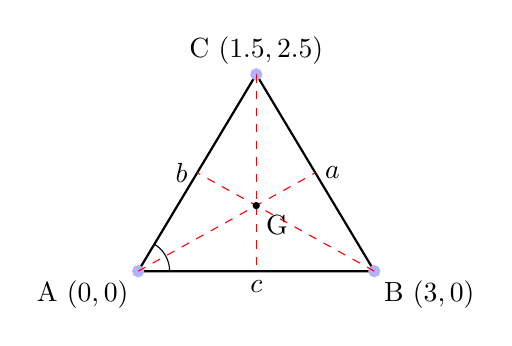
\begin{tikzpicture}
    % Example figure: labeled triangle with details

    % Draw triangle
    \draw[thick] (0,0) -- (3,0) -- (1.5,2.5) -- cycle;

    % Fill vertices
    \filldraw[blue!30!white] (0,0) circle (2pt);
    \filldraw[blue!30!white] (3,0) circle (2pt);
    \filldraw[blue!30!white] (1.5,2.5) circle (2pt);

    % Label vertices
    \node[below left] at (0,0) {A $(0,0)$};
    \node[below right] at (3,0) {B $(3,0)$};
    \node[above] at (1.5,2.5) {C $(1.5,2.5)$};

    % Name the sides
    \node[below] at (1.5,0) {$c$};
    \node[right] at (2.25,1.25) {$a$};
    \node[left] at (0.75,1.25) {$b$};

    % Draw medians
    \draw[dashed, red] (1.5,2.5) -- (1.5,0);
    \draw[dashed, red] (0,0) -- (2.25,1.25);
    \draw[dashed, red] (3,0) -- (0.75,1.25);

    % Mark centroid
    \filldraw[black] (1.5,0.833) circle (1.1pt);
    \node[below right] at (1.5,0.833) {G};

    % Show right angle at vertex A (if assumed)
    \draw (0.4,0) arc (0:60:0.4);

    \end{tikzpicture}
    \caption{A labeled triangle with details}
    \label{fig:triangle}
\end{figure}
% \listnotes
\bibliography{../ref}

\end{document}

